\documentclass[leqno, letterpaper]{article}
\usepackage{geometry}
 \geometry{
 letterpaper,
 left=10mm,
 right=50mm,
 headsep=15mm,
 footskip=0mm,
 }
\usepackage{amsmath}
\usepackage[utf8]{inputenc}
\usepackage{tikz}
\usepackage{marginnote}
\usepackage{setspace}
\usepackage{graphicx}
\usepackage{fancyhdr}
\usepackage{color}
\usepackage{xcolor}
	\definecolor{nocRed}{HTML}{df769b}
	\definecolor{nocOrange}{HTML}{e66533}
	\definecolor{nocYellow}{HTML}{d5971a}
	\definecolor{nocGreen}{HTML}{49e9a6}
	\definecolor{nocGreen2}{HTML}{16b673}
	\definecolor{nocBlue}{HTML}{16a3b6}
	\definecolor{nocBlue2}{HTML}{49ace9}
	\definecolor{nocBlue3}{HTML}{5b858b}
	\definecolor{nocBlue4}{HTML}{7060EB}
	\definecolor{nocBrown}{HTML}{d67e5c}
	\definecolor{gitRed}{HTML}{bd2c00}
	\definecolor{gitOrange}{HTML}{c9510c}
	\definecolor{gitGreen}{HTML}{6cc644}
	\definecolor{gitBlue}{HTML}{4078c0}
	\definecolor{gitPurple}{HTML}{6e5494}
	\definecolor{gitGray1}{HTML}{f5f5f5}
	\definecolor{gitGray2}{RGB}{51,3,0}
\usepackage{multicol}
	\setlength{\columnseprule}{1pt}
	\def\columnseprulecolor{\color{black}}

\newcommand*{\mybox}[1]{\framebox{#1}}


\begin{document}
\pagestyle{fancy}
\fancyhead{}\fancyfoot{}
\renewcommand{\headruleskip}{0mm}
\fancyhead[C]{\begin{center}\huge Physical Science Reference Sheet\end{center}}
\marginnote{
	\setstretch{1.5}
	\begin{center}\Large\mybox{~Variables~}\normalsize\end{center}
	\begin{align*}
		\textcolor{gitRed}{a_{gravity}} & \textcolor{gitRed}{= 10~\frac{meters}{seconds~^2}} \\
		\textcolor{nocBlue2}{m}         & \textcolor{nocBlue2}{~= Mass}                      \\
		\textcolor{gitRed}{D}           & \textcolor{gitRed}{= Density}                      \\
		\textcolor{nocBlue2}{V}         & \textcolor{nocBlue2}{= Volume}                     \\
		\textcolor{gitRed}{~_1}         & \textcolor{gitRed}{= Beginning}                    \\
		\setstretch{0.25}
		\textcolor{gitRed}{}            & \textcolor{gitRed}{~~~~~~~~or}                     \\
		\textcolor{gitRed}{}            & \textcolor{gitRed}{~~~~Initial}                    \\
		\textcolor{nocBlue2}{~_2}       & \textcolor{nocBlue2}{= Ending}                     \\
		\textcolor{nocBlue2}{}          & \textcolor{nocBlue2}{~~~~~~~~or}                   \\
		\textcolor{nocBlue2}{}          & \textcolor{nocBlue2}{~~~~Final}                    \\
		\setstretch{1.5}
		\textcolor{gitRed}{P}           & \textcolor{gitRed}{= Pressure}                     \\
		\textcolor{nocBlue2}{T}         & \textcolor{nocBlue2}{= Temperature}                \\
		\textcolor{gitRed}{E}           & \textcolor{gitRed}{= Energy}                       \\
		\textcolor{nocBlue2}{c}         & \textcolor{nocBlue2}{= Specific~Heat}              \\
		\textcolor{gitRed}{x}           & \textcolor{gitRed}{= Position}                     \\
		\textcolor{nocBlue2}{t}         & \textcolor{nocBlue2}{= Time}                       \\
		\textcolor{gitRed}{a}           & \textcolor{gitRed}{= Acceleration}                 \\
		\textcolor{nocBlue2}{p}         & \textcolor{nocBlue2}{= Momentum}                   \\
		\textcolor{gitRed}{F}           & \textcolor{gitRed}{= Force}                        \\
		\setstretch{0.5}
		\textcolor{nocBlue2}{\mu}       & \textcolor{nocBlue2}{= Coefficient}                \\
		                                & \textcolor{nocBlue2}{~~~~~~~~of}                   \\
		                                & \textcolor{nocBlue2}{~~~~Friction}                 \\
		\setstretch{2}
		\textcolor{gitRed}{W}           & \textcolor{gitRed}{= Work}                         \\
		\textcolor{nocBlue2}{h}         & \textcolor{nocBlue2}{= Height}                     \\
		\textcolor{gitRed}{f}           & \textcolor{gitRed}{= Frequency}                    \\
		\textcolor{nocBlue2}{\lambda}   & \textcolor{nocBlue2}{= Wavelength}                 \\
		\textcolor{gitRed}{I}           & \textcolor{gitRed}{= Current}                      \\
		\textcolor{nocBlue2}{R}         & \textcolor{nocBlue2}{= Resistance}                 \\
	\end{align*}


}
\fancyfoot[C]{
	\begin{center}\Large\mybox{~Units~}\normalsize\end{center}
	\large
	\begin{multicols}{4}
		\textcolor{orange}{
			Mass:~ \(g\) , \(kg\)
		}

		\textcolor{black}{
			Volume:~ \(mL\) , \(L\)
		}

		\textcolor{orange}{
			Density:~ \(cm^3\) , \(\frac{g}{mL}\) , \(\frac{kg}{mL}\)
		}

		\textcolor{black}{
			Pressure:~ \(atm\) , \(psi\) , \(torr\) , \(mmHg\)
		}

		\textcolor{orange}{
			Force:~ \(N\)
		}

		\textcolor{black}{
			Area:~ \(cm^2\) , \(m^2\)
		}

		\textcolor{orange}{
			Temperature:~ \(K\) , \(^{\circ}\)C , \(^{\circ}\)F
		}

		\textcolor{black}{
			Energy:~ \(J\)
		}

		\textcolor{orange}{
			Velocity:~ \(\frac{m}{s}\)
		}


		\textcolor{black}{
			Time:~ \(s\)
		}

		\textcolor{orange}{
			Acceleration:~\(\frac{cm}{s^2}\) , \(\frac{m}{s^2}\)
		}

		\textcolor{black}{
			Momentum:~ \(kg\cdot\frac{m}{s^2}\)
		}

		\textcolor{orange}{
			Work:~ \(N\cdot m\) , \(J\)
		}

		\textcolor{black}{
			Power:~ \(W\)
		}


		\textcolor{orange}{
			Frequency:~ \(Hz\)
		}

		\textcolor{black}{
			Voltage:~ \(V\)
		}

		\textcolor{orange}{
			Current:~ \(A\)
		}

		\textcolor{black}{
			Resistance:~ \(\Omega\)
		}

		\textcolor{orange}{
			Position or Distance:~ \(cm\) , \(m\) , \(km\)
		}
	\end{multicols}
}

\begin{center}\Large\mybox{~Formulas~}\normalsize\end{center}
\bigskip
\setstretch{0.5}
\begin{multicols}{3}

	\begin{center}\underline{Density}\end{center}
	\textcolor{nocRed}{
		\begin{equation}
			D = \frac{m}{V}
		\end{equation}
	}

	\begin{center}\underline{Pressure}\end{center}
	\textcolor{nocOrange}{
		\begin{equation}
			P = \frac{F}{A}
		\end{equation}
	}

	\begin{center}\underline{Boyle's Law}\end{center}
	\textcolor{nocYellow}{
		\begin{subequations}\label{boyle:main}
			\begin{equation}
				P_1 \cdot V_1 = P_2 \cdot V_2 \tag{\ref{boyle:main}}
			\end{equation}
			\begin{equation}
				P_1 = \frac{P_2 \cdot V_2}{V_1} \label{boyle:a}
			\end{equation}
			\begin{equation}
				V_1 = \frac{P_2 \cdot V_2}{P_1} \label{boyle:b}
			\end{equation}
			\begin{equation}
				P_2 = \frac{P_1 \cdot V_1}{V_2} \label{boyle:c}
			\end{equation}
			\begin{equation}
				V_2 = \frac{P_1 \cdot V_1}{P_2} \label{boyle:d}
			\end{equation}
		\end{subequations}
	}

	\begin{center}\underline{Charles's Law}\end{center}
	\textcolor{nocGreen2}{
		\begin{subequations}\label{charles:main}
			\begin{equation}
				\frac{V_1}{T_1}=\frac{V_2}{T_2} \tag{\ref{charles:main}}
			\end{equation}
			\begin{equation}
				V_1 = \frac{V_2 \cdot T_1}{T_2} \label{charles:a}
			\end{equation}
			\begin{equation}
				T_1 = \frac{V_1 \cdot T_2}{V_2} \label{charles:b}
			\end{equation}
			\begin{equation}
				V_2 = \frac{V_1 \cdot T_2}{T_1} \label{charles:c}
			\end{equation}
			\begin{equation}
				T_2 = \frac{V_2 \cdot T_1}{V_1} \label{charles:d}
			\end{equation}
		\end{subequations}
	}

	\begin{center}\underline{Gay-Lussac's Law}\end{center}
	\textcolor{nocBlue}{
		\begin{subequations}\label{gl:main}
			\begin{equation}
				\frac{P_1}{T_1}=\frac{P_2}{T_2} \tag{\ref{gl:main}}
			\end{equation}
			\begin{equation}
				P_1 = \frac{P_2 \cdot T_1}{T_2} \label{gl:a}
			\end{equation}
			\begin{equation}
				T_1 = \frac{P_1 \cdot T_2}{P_2} \label{gl:b}
			\end{equation}
			\begin{equation}
				P_2 = \frac{P_1 \cdot T_2}{T_1} \label{gl:c}
			\end{equation}
			\begin{equation}
				T_2 = \frac{P_2 \cdot T_1}{P_1} \label{gl:d}
			\end{equation}
		\end{subequations}
	}

	\begin{center}\underline{Specific Heat}\end{center}
	\textcolor{nocBrown}{
		\begin{equation}
			E = m \cdot c \cdot (T_2 - T_1)
		\end{equation}
	}

	\begin{center}\underline{Velocity}\end{center}
	\textcolor{gitPurple}{
		\begin{equation}
			v = \frac{x_2 - x_1}{t_2 - t_1}
		\end{equation}
	}

	\begin{center}\underline{Acceleration}\end{center}
	\textcolor{gitRed}{
		\begin{equation}
			a = \frac{v_2 - v_1}{t_2 - t_1}
		\end{equation}
	}

	\begin{center}\underline{Momentum}\end{center}
	\textcolor{gitOrange}{
		\begin{equation}
			p = m \cdot v
		\end{equation}
	}

	\begin{center}\underline{Force}\end{center}
	\textcolor{gitGreen}{
		\begin{subequations}\label{force:main}
			\begin{equation}
				F_{net} = m \cdot a \tag{\ref{force:main}}
			\end{equation}
			\begin{equation}
				Weight = m \cdot a_{gravity}\label{force:a}
			\end{equation}
			\begin{equation}
				F_{friction} = \mu \cdot F_{normal}
			\end{equation}
		\end{subequations}
	}

	\begin{center}\underline{Work}\end{center}
	\textcolor{gitBlue}{
		\begin{equation}
			W = F_{net} \cdot (x_2 - x_1)
		\end{equation}
	}

	\begin{center}\underline{Power}\end{center}
	\textcolor{gitPurple}{
		\begin{equation}
			Power = \frac{W}{t}
		\end{equation}
	}

	\begin{center}\underline{Energy}\end{center}
	\textcolor{gitRed}{
		\begin{equation}
			E_{kinetic} = \frac{1}{2}\cdot m \cdot v^2
		\end{equation}
		\begin{equation}
			E_{gravity} = m \cdot a_{gravity} \cdot h
		\end{equation}
	}

	\begin{center}\underline{Waves}\end{center}
	\textcolor{gitOrange}{
		\begin{equation}
			v_{wave} = f \cdot \lambda
		\end{equation}
	}

	\begin{center}\underline{Electricity}\end{center}
	\textcolor{gitGreen}{
		\begin{equation}
			Voltage = I \cdot R
		\end{equation}
	}
\end{multicols}
\newpage
\renewcommand{\headrulewidth}{0pt}
\textcolor{white}{Periodic Table}
\AddToHookNext{shipout/background}{
	\begin{tikzpicture}[remember picture,overlay]
		\node at (current page.center) {
			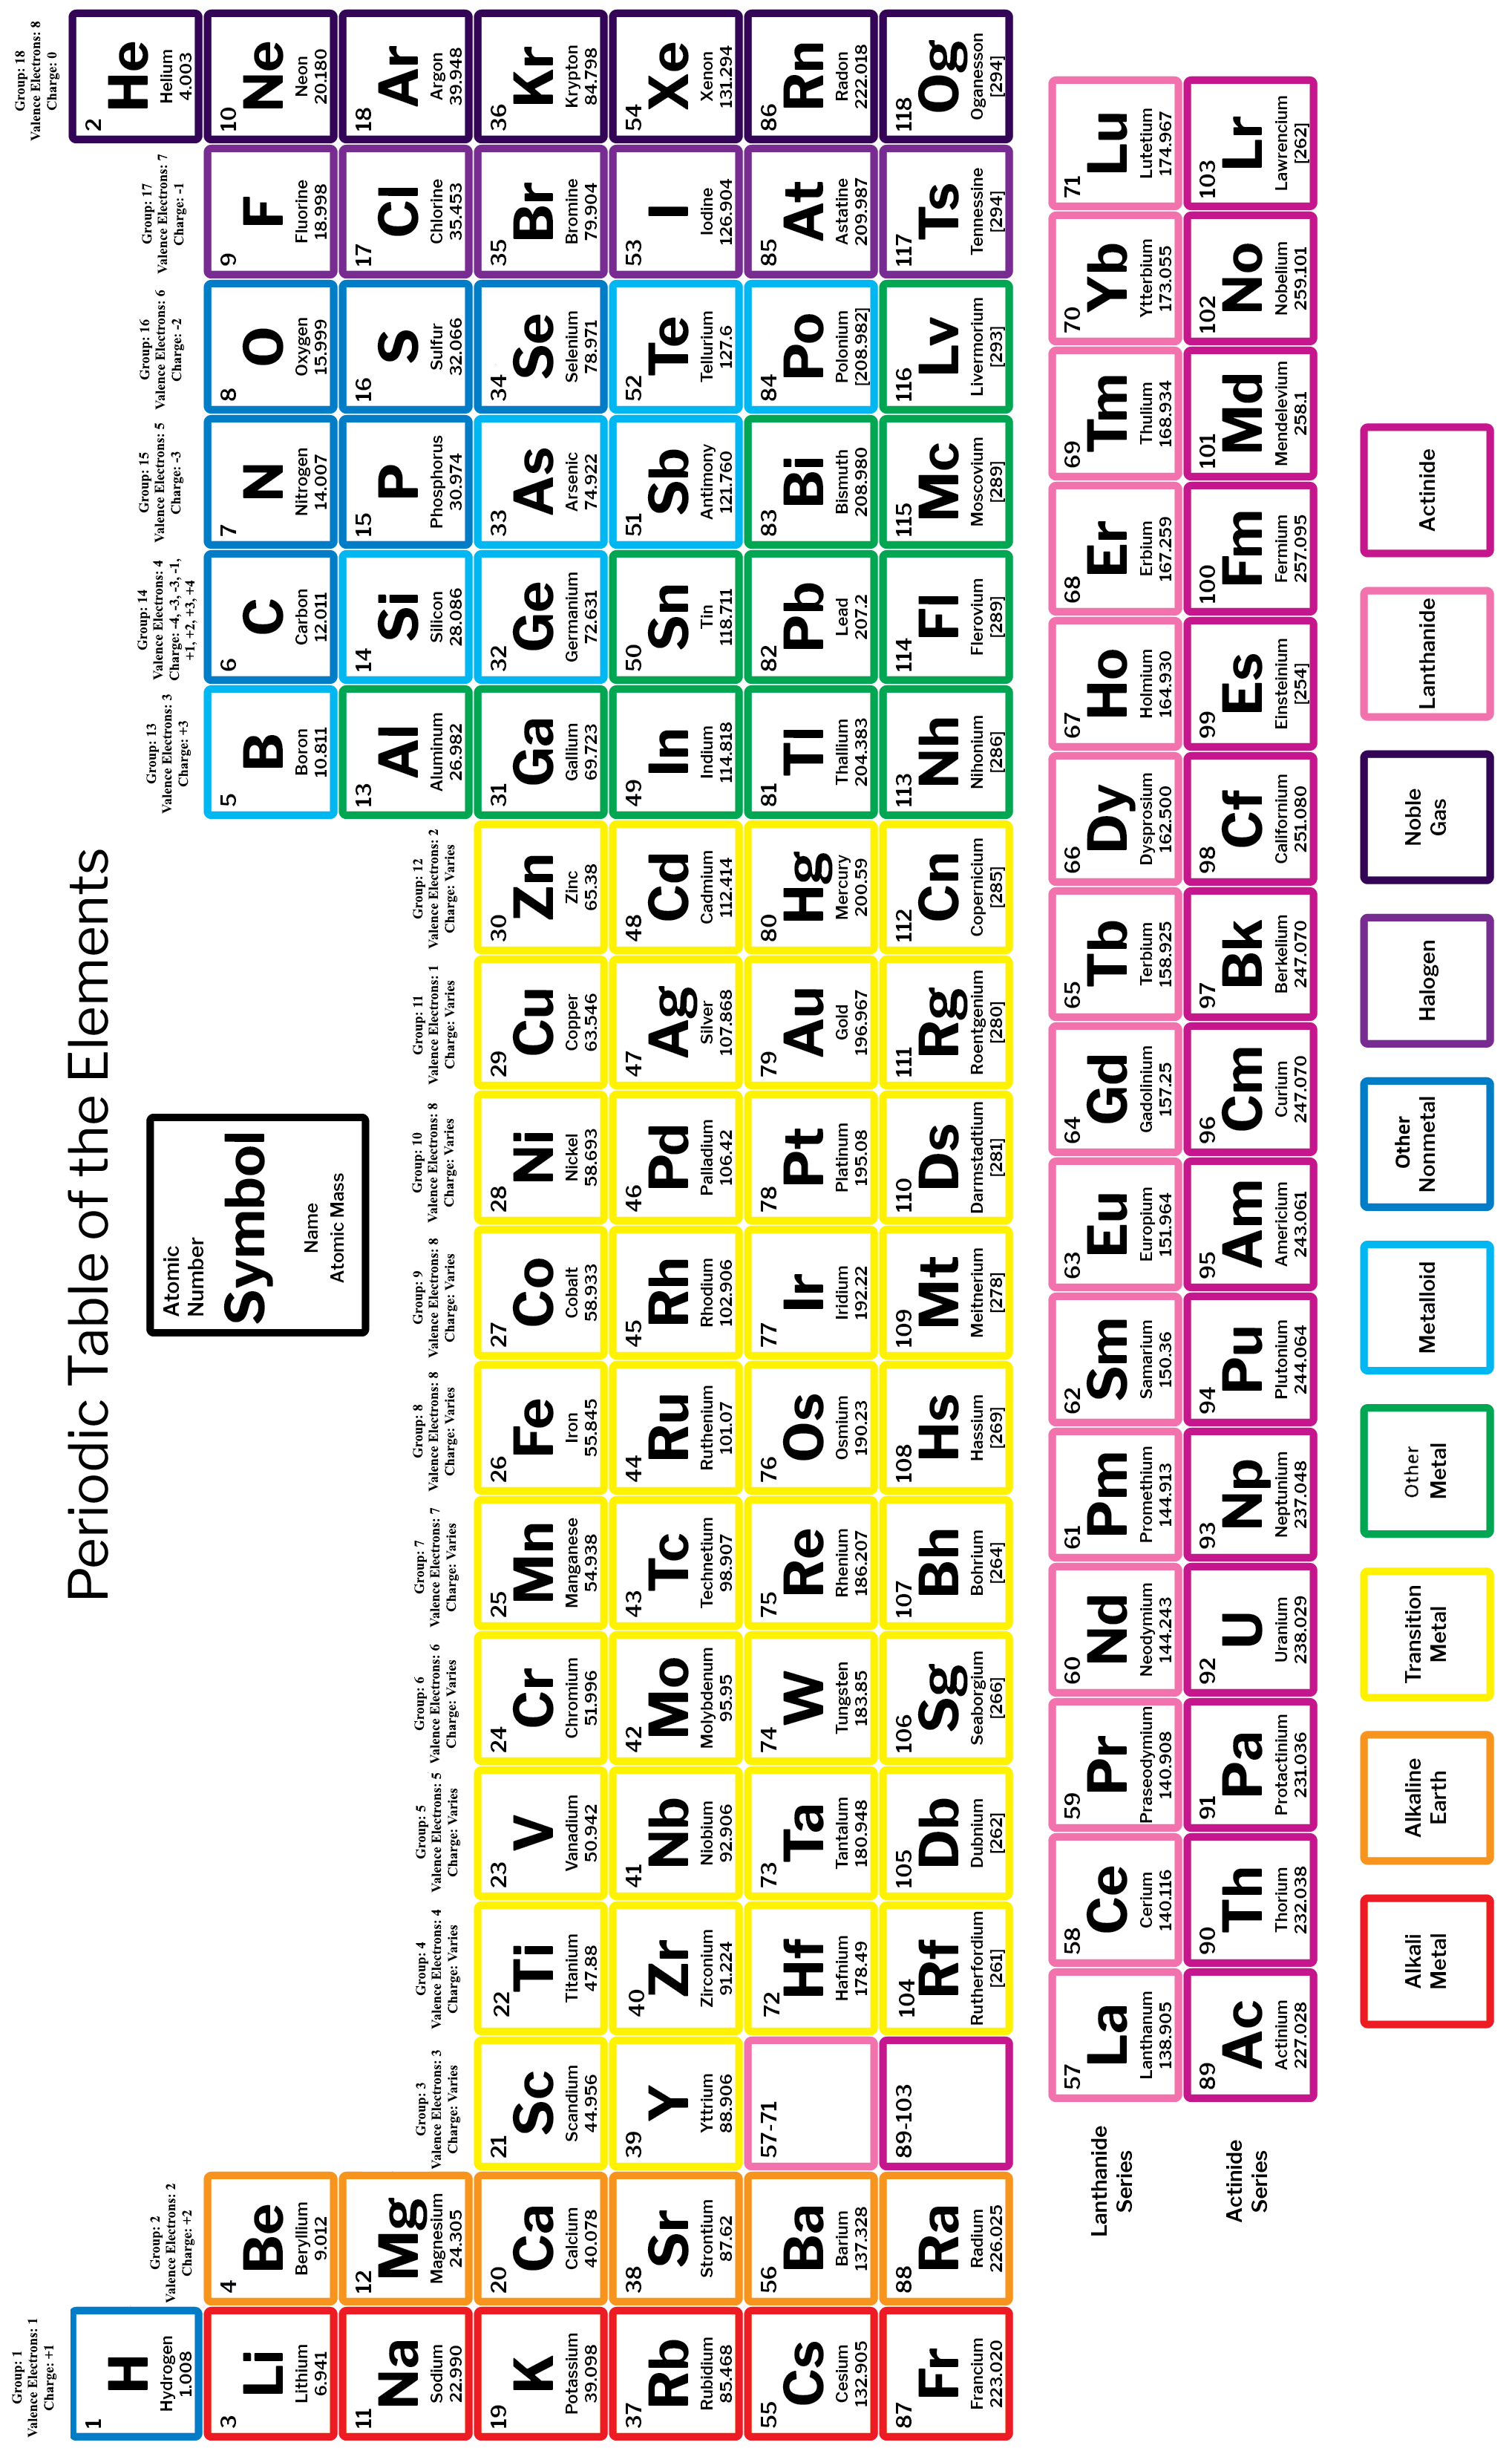
\includegraphics[width=16cm]{Periodic_Table.png}
		};
	\end{tikzpicture}
}
\fancyfoot{}
\fancyhead[]{}
\end{document}
